\documentclass{article}
\usepackage{enumitem}
\usepackage{geometry}
\usepackage{graphicx}
\usepackage{url}
\usepackage{hyperref}
\usepackage[spanish]{babel}
\usepackage{parskip}
\usepackage{amssymb}
\usepackage{amsmath}
\usepackage{mathtools}
\usepackage{listings}
\usepackage{xcolor}
\lstset{
    language=Python,
    basicstyle=\ttfamily\small,
    keywordstyle=\color{blue},
    stringstyle=\color{green!60!black},
    commentstyle=\color{gray},
    numbers=left,
    numberstyle=\tiny\color{gray},
    stepnumber=1,
    numbersep=5pt,
    showstringspaces=false,
    frame=single,
    rulecolor=\color{black!30},
    tabsize=4,
    backgroundcolor=\color{gray!10}
}




\title{Examen 3: Detector de objetos con DNN OPENCV}

\author{
  \begin{minipage}[t]{0.4\linewidth}
    \centering
    Quistian Navarro, Juan Luis\\
    A341807@alumnos.uaslp.mx 
  \end{minipage}
}
\date{\today}
\begin{document}

\maketitle

\begin{minipage}{\textwidth}
    \centering
    \textit{Ing. Sistemas Inteligentes, Gen. 2021} \\
    \textit{Visión Computacional}
\end{minipage}

\small
\section{Planteamiento del problema}
Implementar un Detector de objetos  utilizando el módulo DNN de Opencv:

\begin{enumerate}[label=\alph*)]
    \item Investigar sobre el dataset de Imágenes de objetos MS COCO. Decir quién y cuándo lo creó. Qué
    contiene, cuantas clases y número de imágenes. Agregar para que tipo de problemas se ha utilizado
    y el enlace de donde se puede bajar públicamente. Finalmente, mencione otros 3 datasets utilizados
    popularmente para la detección de objetos.
    \item Utilizar la biblioteca OpenCV para implementar un programa que detecte objetos que pertenezcan
    a alguna(s) de clase(s) del dataset MS COCO. Para ello puede basarse en el ejercicio que vimos
    en clase. Para el programa que usted realice, puede utilizar cualquiera de las DNN y frameworks
    soportados que vienen en la documentación de OpenCV. Pero para obtener un buen desempeño,
    debería asegurarse que la DNN que elija está ya pre-entrenada con el dataset MS COCO.
    \item Para probar su implementación, debe tomar una foto (o video, si su capacidad de cómputo lo
    permite) usted mismo donde aparezcan objetos de las clases de MS COCO. Si es muy difícil hacer
    una foto o video con las clases que usted eligió para probar, puede utilizar alguna imagen o video
    del dominio público y poner la referencia de donde lo obtuvo. El caso es que NO utilice fotos o
    videos del dataset MS COCO
\end{enumerate}
\section{Descripción de la solución}

\subsection{Dataset MS COCO}
% quien lo creo y cuando
% que contiene
% cuantas clases 
% numero de results_lg/Figure_es%n para que tipo de prblemas se ha utilizado
% enlace donde se puede bajar públicamente

Microsoft Common Objects in Context (MSCOCO) \cite{lin2015microsoftcococommonobjects}, fue creado por Microsoft en 2014, presentado por Lin et al. Se ha utilizado ampliamente en investigaciones sobre 
detección de objetos, segmentación y captioning. Este dataset contiene más de 200,000 imágenes etiquetadas, con más de 80 clases de objetos diferentes. Cada imagen
está etiquetada con los objetos que contiene, junto con sus coordenadas de localización y máscaras de segmentación en algunos casos \cite{lin2015microsoftcococommonobjects}.

COCO es un dataset desafiante debido a la gran variabilidad en las condiciones de las imágenes, como cambios de escala, rotación y contexto visual. Se ha utilizado
 en diversas competiciones de detección de objetos y es uno de los estándares para evaluar modelos en tareas de visión computacional.

Para obtener el dataset, se puede acceder públicamente en el siguiente enlace: \url{http://cocodataset.org/}.

\subsection{Otros datasets}
Además del dataset COCO, exiten otros datasetscomunes en la investigación en visión computacional,como el PASCAL VOC \cite{Everingham15} cuya última versión consiste en 11k imágenes de entrenamiento
con 20 clases de objetos diferentes, ImageNet Large Scale Visual Recognition Challenge (ILSVRC) \cite{russakovsky2015imagenetlargescalevisual} dataset que toma un subconjunto del más de un millon de imágenes con 1000
categorías para clasificación y Open Images dataset de Google \cite{Kuznetsova_2020}, que esta compuesto por 9 millones de imágenes con 6000 categorías de objetos \cite{zaidi2021surveymoderndeeplearning}.

\section{Mask R-CNN Inception V2 (entrenado con MSCOCO)}
% quien la propuso 
% descripción de la arquitectura
% para que probelema se propuso

Mask R-CNN fue propuesto por He et al. en 2017 \cite{he2018maskrcnn}, como una extensión de Faster R-CNN. Mientras que Faster R-CNN \cite{girshick2015fastrcnn} 
se enfoca en la detección y clasificación de objetos, Mask R-CNN añade una rama adicional para la segmentación de objetos, lo que permite obtener una máscara precisa de 
cada objeto en la imagen.

\begin{figure}[!ht]
    \centering
    \includegraphics[width=0.76\textwidth]{results_lg/maskrcnn.png}
    \caption{Arquitectura de Mask R-CNN}
    \label{fig:mask_rcnn}
\end{figure}

La arquitectura Mask R-CNN \ref{fig:mask_rcnn} se basa en la red Inception V2, que es una variante de las redes convolucionales profundas que busca optimizar el uso
de recursos computacionales manteniendo un buen desempeño en tareas de clasificación y detección. Inception V2 es conocida por su capacidad para 
detectar patrones a diferentes escalas de forma eficiente, lo cual es esencial en la detección de objetos en imágenes complejas.

Mask R-CNN es una solución robusta y flexible, adecuada para problemas de detección y segmentación de objetos en diversas aplicaciones como 
la robótica, la vigilancia, la conducción autónoma, y más.

\subsection{Implementación}
El modelo utilizado para la detección es una versión pre-entrenada de Mask R-CNN basada en el modelo Inception V2, entrenado con el dataset COCO, obteniendo
los archivos de configuración del repositorio en github emugcv\cite{emgucv_models} y de Open\_extra \cite{opencv_extra}.
\subsubsection{Funciones de OpenCV}
OpenCV proporciona diversas funciones para cargar modelos pre-entrenados y realizar inferencias sobre imágenes. A continuación se detalla el flujo 
principal del código usado para cargar y ejecutar la red Mask R-CNN, codigo basado en \cite{canu2021instance}:

\begin{lstlisting}
  # Cargar el modelo Mask R-CNN
  net = cv2.dnn.readNetFromTensorflow(MODEL_PATH, CONFIG_PATH)

  def net_inference(net, image, labels_coco,true_label, threshold=0.5):
  # Preparar la imagen de entrada
    blob = cv2.dnn.blobFromImage(image, swapRB=True)
  # Establecer la imagen como entrada a la red
    net.setInput(blob)
  # Realizar la inferencia para obtener cajas de deteccion y mascaras
    boxes, _ = net.forward(["detection_out_final", "detection_masks"])
    detection_count = boxes.shape[2]
    detections = []

    for i in range(detection_count):
        box = boxes[0, 0, i]
        class_id = int(box[1])  
        confidence = box[2]

        if confidence > threshold:
            if 0 <= class_id < len(labels_coco):  
                label = labels_coco[class_id]
                x = int(box[3] * image.shape[1]) 
                y = int(box[4] * image.shape[0])
                x2 = int(box[5] * image.shape[1])
                y2 = int(box[6] * image.shape[0])
                
                if label == true_label:
                    detections.append({
                        "label": label,
                        "bbox": (x, y, x2, y2),
                        "confidence": confidence
                    })
            else:
                print(f"Warning: class_id {class_id} is out of
                 range for labels_coco")
    return detections
\end{lstlisting}
  
\begin{enumerate}
  \item \textbf{Cargar el modelo}: `cv2.dnn.readNetFromTensorflow(MODEL\_PATH, CONFIG\_PATH)` carga un modelo TensorFlow utilizando su gráfico congelado (`frozen\_inference\_graph.pb`) y archivo de configuración.
  \item \textbf{Preparar la imagen de entrada}: `cv2.dnn.blobFromImage(image, swapRB=True)` convierte la imagen en un blob, que es el formato que las redes DNN utilizan para realizar inferencias.
  \item \textbf{Configurar la entrada}: `net.setInput(blob)` alimenta el blob a la red.
  \item \textbf{Inferencia}: `net.forward` ejecuta la inferencia para obtener las cajas de detección y máscaras de los objetos identificados.
  
\end{enumerate}

Este flujo garantiza que la red procese correctamente la imagen de entrada y genere predicciones en términos de cajas de delimitación y segmentaciones.

\subsubsection{Parámetros de configuración}
La implementación del modelo Mask R-CNN requiere configurar correctamente los siguientes parámetros:

\begin{itemize}
    \item \textbf{MODEL\_PATH}: Ruta al archivo del modelo pre-entrenado (\textit{frozen\_inference\_graph.pb}), que contiene los pesos entrenados de la red.
    \item \textbf{CONFIG\_PATH}: Ruta al archivo de configuración (\textit{mask\_rcnn\_inception\_v2\_coco.pbtxt}), que describe la arquitectura de la red y las clases de salida.
    \item \textbf{swapRB}: Especifica si se debe intercambiar los canales Rojo y Azul de la imagen de entrada. Esto es común en modelos entrenados con TensorFlow, ya que utilizan el formato BGR.
    \item \textbf{Output Layers}: Capas específicas de salida de la red, como \textit{"detection\_out\_final"} (para las cajas) y \textit{"detection\_masks"} (para las máscaras).
\end{itemize}

Estos parámetros son fundamentales para garantizar que el modelo funcione correctamente.

\section{Resultados}
Para evaluar el desempeño del modelo, decidí  utilizar las imágenes del dataset PASCAL VOC que descargue de roboflow \cite{pascal_voc_2012} en el formato coco json, que es un archivo que tiene el formato similar al dataset baby coco.
Debo mencionar que PASCAL VOC tiene los bounding boxes en formato x, y, w, h y la red maskrcnn devuelve los bounding boxes en formato x1,y1,x2,y2 asi que tuve que pasarlo a ese formato al hacer la carga de imagenes. PASCAL VOC 
contiene clases de objetos similares a las de COCO, elegí cat, dog, bird y horse. 
Se limitó el numero de imagenes por cada clase a un maximo de 100 imagenes para probar el modelo.
Las figura \ref{fig:results} muestra las predicciones del modelo sobre las imágenes de prueba.
% \newpage
% \subsection{Visualización de resultados}
% En la figura \ref{fig:results} podemos observar algunos resultados de las clases detectadas en las imagenes usada de PASCAL VOC. 
\begin{figure}[htbp]
  \centering
  % Primera fila
  \begin{minipage}{0.24\textwidth}
      \centering
      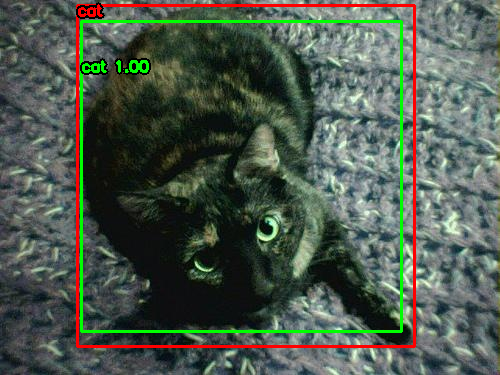
\includegraphics[width=\linewidth]{results_lg/cat_0.png}
  \end{minipage}
  \begin{minipage}{0.24\textwidth}
      \centering
      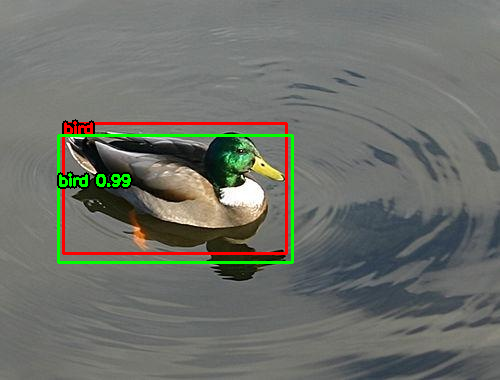
\includegraphics[width=\linewidth]{results_lg/bird_57.png}
  \end{minipage}
  \begin{minipage}{0.24\textwidth}
      \centering
      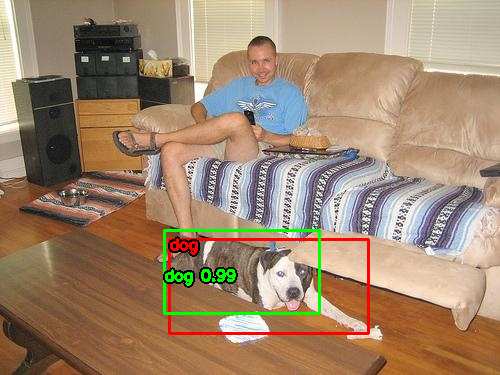
\includegraphics[width=\linewidth]{results_lg/dog_0.png}
  \end{minipage}
  \begin{minipage}{0.24\textwidth}
      \centering
      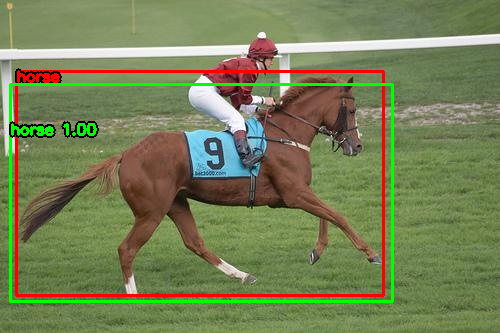
\includegraphics[width=\linewidth]{results_lg/horse_1.png}
  \end{minipage}
  
  % Segunda fila
  \vspace{0.5cm} % Espacio entre filas
  \begin{minipage}{0.24\textwidth}
      \centering
      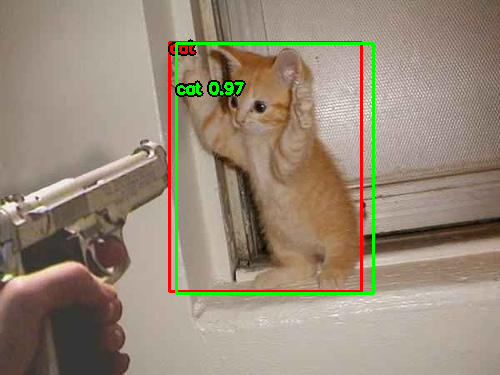
\includegraphics[width=\linewidth]{results_lg/cat_16.png}
  \end{minipage}
  \begin{minipage}{0.24\textwidth}
      \centering
      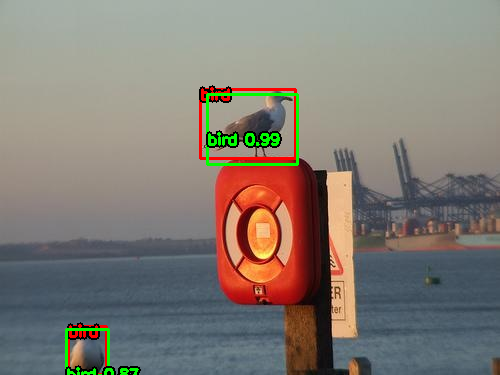
\includegraphics[width=\linewidth]{results_lg/bird_3.png}
  \end{minipage}
  \begin{minipage}{0.24\textwidth}
      \centering
      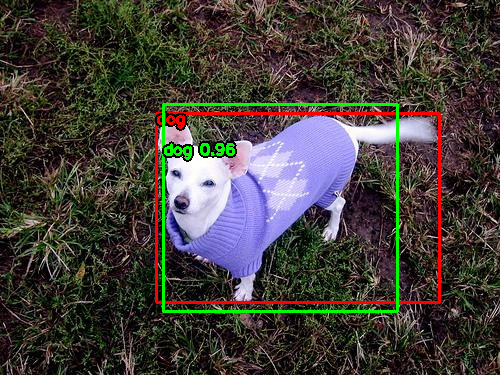
\includegraphics[width=\linewidth]{results_lg/dog_44.png}
  \end{minipage}
  \begin{minipage}{0.24\textwidth}
      \centering
      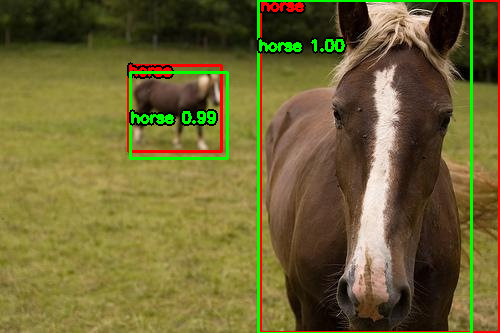
\includegraphics[width=\linewidth]{results_lg/horse_42.png}
  \end{minipage}
  
  \caption{Resultados de las clases: cat, bird, dog, horse (Bbox rojo es el ground truth, bbox verde es la predicción)}
  \label{fig:results}
\end{figure}

\subsection{Mean Average Precision}
El desempeño del modelo se evaluó utilizando la métrica de Mean Average Precision (mAP) \cite{henderson2017endtoendtrainingobjectclass}, que es una de las métricas más utilizadas en la detección de objetos. 
El mAP se calcula para diferentes umbrales de Intersection over Union (IoU), y representa el promedio de la precisión de las detecciones en diferentes niveles de recall.
Generalmente, el mAP toma valores en el rango de [0, 1], donde:

\begin{itemize}
  \item 0 indica que el modelo no es capaz de recuperar correctamente ningún elemento relevante.
  \item 1 indica que el modelo recupera todos los elementos relevantes con perfecta precisión en todas las clases o consultas.
\end{itemize}

\section{Intersection over Union}
Intersection over Union (IoU) \cite{padilla2020survey} es una métrica utilizada en visión por computadora para evaluar la precisión de modelos de detección de objetos. Calcula la
superposición entre el área de intersección y el área de unión de dos regiones: la predicción del modelo y la verdera. La formula es la siguiente: 
\[
\text{IoU} = \frac{|A \cap B|}{|A \cup B|}
\]

Donde \( A \) es el área predicha y \( B \) el área de la verdad real (ground truth). \( |A \cap B| \) representa el área de intersección y \( |A \cup B| \) el área de unión.
El cálculo del Intersection over Union (IoU) es fundamental para evaluar la precisión de las detecciones en términos de la superposición entre las cajas de delimitación predichas y las reales.
En la figura \ref{fig:mAP} se presenta el gráfico que muestra cómo el mAP varía en función del umbral de IoU.
A mayor IoU, se espera que las detecciones sean más precisas, ya que se requiere una mayor superposición entre las cajas de delimitación predichas y las reales, y como podemos observar el mAP disminuye
si el IoU es muy alto, incluso llegando a cero.

\begin{figure}[!ht]
    \centering
    \includegraphics[width=0.58\textwidth]{results_lg/mAP_vs_IoU.png}
    \caption{Mean Average Precision vs Intersection over Union}
    \label{fig:mAP}
\end{figure}

\section{Discusión}
Los resultados obtenidos muestran que el modelo tiene un desempeño destacado con umbrales bajos de IoU, alcanzando un mAP cercano a 1 a 0.10 de IoU. 
Sin embargo, a medida que el umbral de IoU aumenta, la precisión del modelo disminuye, por lo que el modelo tiende a ser más flexible a menores umbrales de IoU, pero pierde precisión a medida que se requieren coincidencias más exactas entre las predicciones y las cajas de delimitación reales.
Además, el análisis de los resultados visuales muestra que el modelo ha sido capaz de identificar correctamente los objetos en las imágenes de prueba, pero en algunos casos, especialmente en objetos más pequeños o parcialmente visibles, la precisión disminuye.

\section{Conclusión}
El modelo Mask R-CNN Inception V2 ha demostrado ser eficaz para la detección de objetos en imágenes utilizando el dataset PASCAL VOC. 
Los resultados obtenidos sugieren que el modelo es robusto, aunque la precisión disminuye cuando se incrementa el umbral de IoU. 
Parece ser que en imagenes con objetos solapados o parcialmente visibles, el modelo tiene dificultades para identificar los objetos correctamente.
Aun así, el modelo es adecuado para cumplir con la deteccion de objetos. 

\bibliographystyle{unsrt}
\bibliography{ref}
\end{document}